\documentclass[10pt,a4paper]{article}
\usepackage[a4paper,left=2cm,right=2cm,top=1.5cm,bottom=1.5cm]{geometry}
\usepackage[utf8]{inputenc}
\usepackage[T1]{fontenc}
\usepackage{amsmath}
\usepackage{amssymb}
\usepackage{graphicx}
\usepackage{abstract}
\usepackage{ctex}
\usepackage[hidelinks]{hyperref} %生成左侧目录,并隐藏目录上的红框
\linespread{1.5} %行距

\begin{document}
% \maketitle %编译标题
\tableofcontents %目录
\newpage

\section{2023-3-23 小论文框架图}
\numberwithin{equation}{section}

\begin{figure}[!htb]
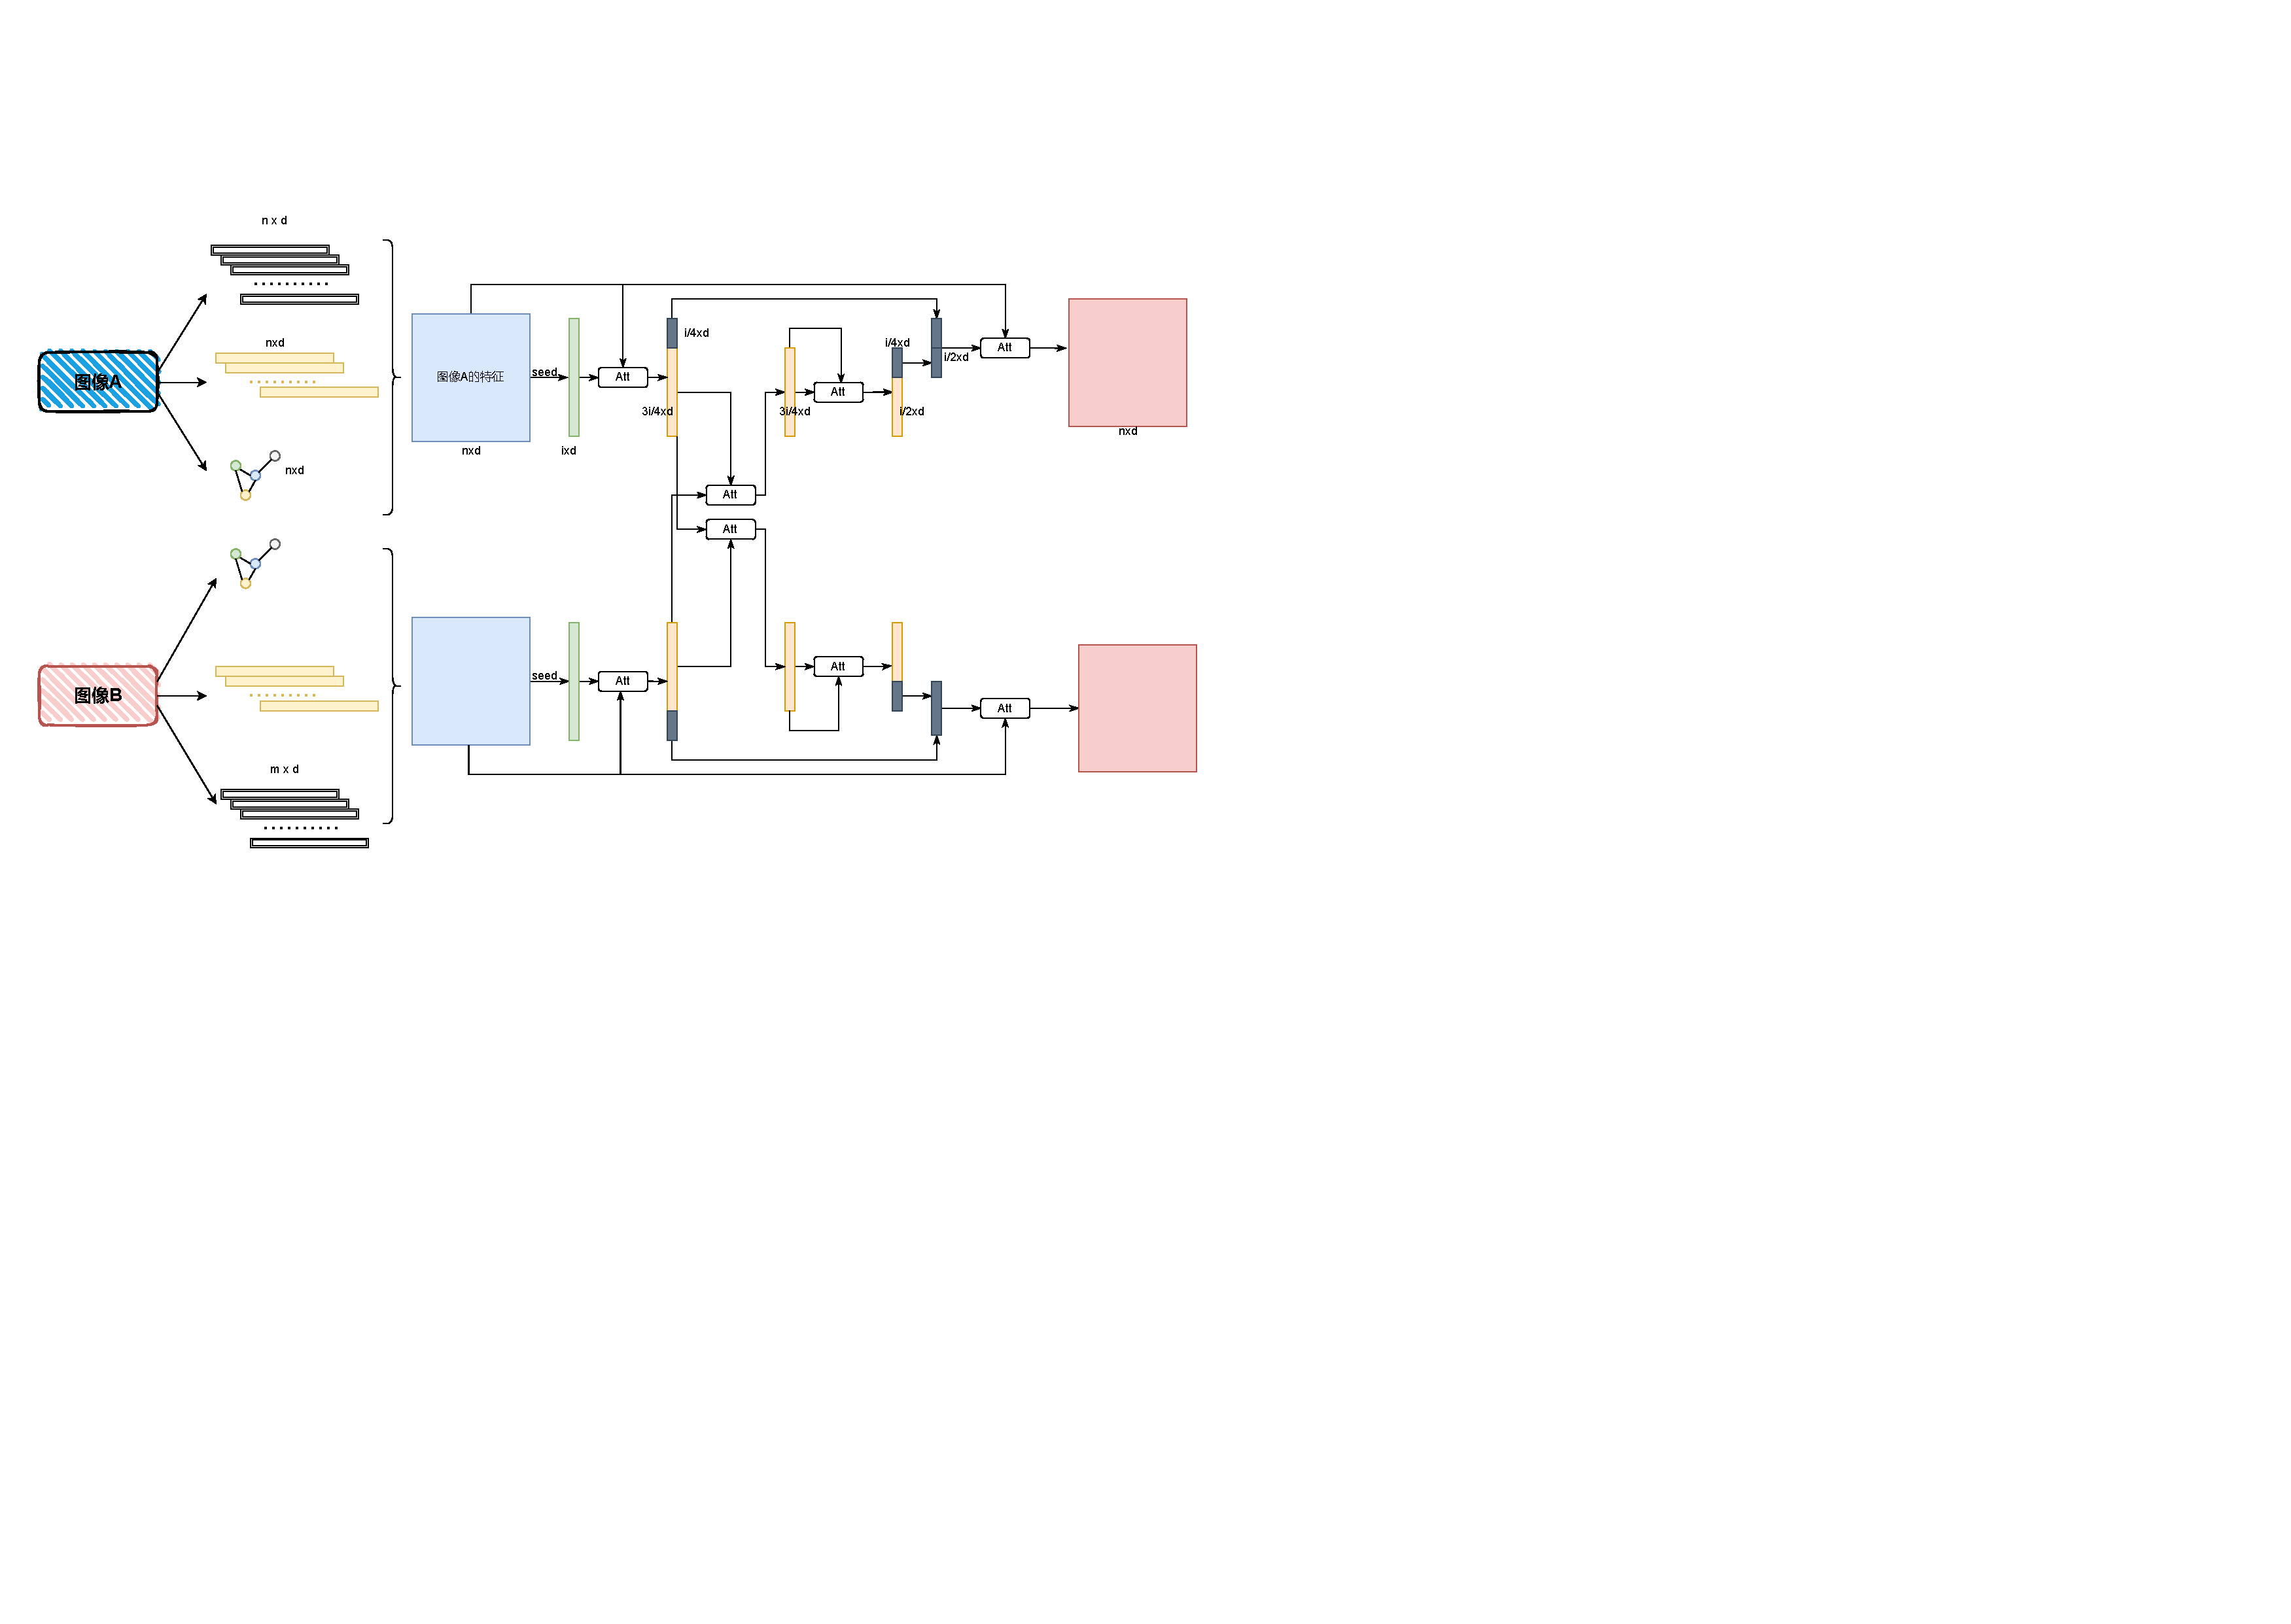
\includegraphics[width=\hsize]{images/论文框图.pdf}
\caption{论文深度学习网络草图}
\end{figure}

学习进展:

1、完成图像特征点领域选取和聚合的代码实现。

邻域:
\begin{align}
   \mathcal{N}_i=\{\mathbf{n}\in \mathbf{topk}(\mathbf{D}_i)\}
\end{align}

聚合方法:也是整个网络采取的一种带权重的注意力机制
\begin{align}
   \mathbf{X}^{'}=\mathbf{\emph{Att}}(\mathbf{X},\mathbf{Y},\mathbf{\omega}) 
\end{align}

2、训练网络设计,大致框图如图1所示。

3、参照其它特征点匹配文章,选取其中的上下文正则化方法作为训练网络不同层匹配点特征的评价函数。正则化在网络中一般是用来减少网络
复杂度,防止梯度消失或爆炸,加速收敛,这个思想也可以用来评价。

4、理解了一下sinkhorn算法用于求解图像之间的分配矩阵。因为图之间的匹配可抽象为二次分配问题,通俗来说就是求解两个样本分布或数据
之间的最短距离,也可用作图像特征点(像素点)之间最优映射求解方法,通过一个迭代算法使得分配矩阵达到收敛或迭代次数。算法的具体步骤
如下:

初始化:给定两个概率分布 $\mu$ 和 $\nu$,初始化一个矩阵 $K$,其中 $K_{i,j} = \exp(-c_{i,j})$,$c_{i,j}$ 是 $\mu$ 中第
$i$ 个元素和 $\nu$ 中第 $j$ 个元素之间的距离,可以是欧几里得距离、马氏距离等。

迭代更新:重复执行以下步骤,直至收敛:

\qquad a. 计算 $\gamma$:$\gamma_{i,j}=\frac{K_{i,j}u_i v_j}{\epsilon+\sum_{i',j'}K_{i',j'}u_{i'}v_{j'}}$,其中 $u$ 和
 $v$ 是两个向量,分别表示从 $\mu$ 和 $\nu$ 出发的概率质量。

\qquad b. 更新 $u$ 和 $v$:$u_i=\frac{\mu_i}{\sum_j K_{i,j}v_j}$,$v_j=\frac{\nu_j}{\sum_i K_{i,j}u_i}$。

输出 $\gamma$。

其中,$\epsilon$ 是一个较小的正数,用于避免分母为零。

下周安排:

1、根据框图完成训练网络的代码实现。

2、理解上下文正则化方法,将其改变为匹配点的评价方法,并实现为一种可训练网络层。

3、实现sinkhorn算法。

4、损失函数设计,除了最基本对于结果和分配矩阵的损失计算(参考论文),需要设计一个对注意力转移的损失函数,约束注意力析出的匹配点为
最优匹配。

\section{FAST_LIO2:Fast Direct LiDAR-inertial Odometry}
\subsection{摘要}
这是一种高效的紧耦合,基于迭代卡尔曼滤波的LIO系统。两个新颖的点:一是直接将数据点与地图配准,然后再进行地图的跟新,
不需要提取特征点,这使得更好的适应环境变化和提高准确率。二是地图的存贮用了一个增量树的数据结构(kd-tree),更高的效率。
\subsection{介绍}
目前LiDAR传感器的优缺点,优点是能够克服环境光照等干扰提供更多的特征信息。缺点是数据量大计算成本高、特征提取的方式容易
丢失一些重要信息、比如再一些环境结构简单的地方,或者LiDAR的FoV小、运动失真,惯性测量单元可以减少影响、点云稀疏分布在
一个大空间的地图,地图需要支持高效的搜索查询。

\end{document}